% Author: Izaak Neutelings (July 2017)
% Timelines & energy scales of particle physics
\documentclass[border=1pt,tikz]{standalone}

\usepackage{amsmath} % for \dfrac
\usepackage{tikz}
\tikzset{>=latex} % for LaTeX arrow head

\begin{document}


% TIMELINE - simple test
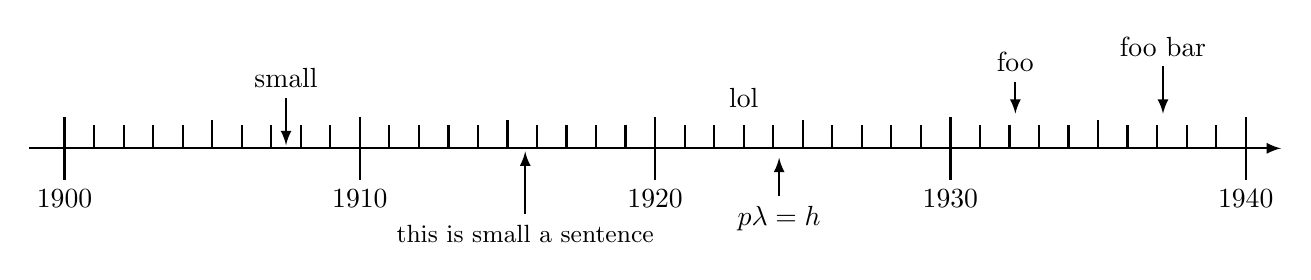
\begin{tikzpicture}[]
  
  % limits
  \newcount\yearOne; \yearOne=1900
  \def\w{15}    % width of axes
  \def\n{4}     % number of decades
  \def\lt{0.40} %  ten tick length
  \def\lf{0.36} % five tick length
  \def\lo{0.30} %  one tick length
  
  % help functions
  \def\yearLabel(#1,#2){\node[above] at ({(#1-\yearOne)*\w/\n/10},\lt) {#2};}
  \def\yearArrowLabel(#1,#2,#3,#4){
    \def\xy{{(#1-\yearOne)*\w/\n/10}}; \pgfmathparse{int(#2*100)};
    \ifnum \pgfmathresult<0
      \def\yyp{{(\lt*(0.90+#2))}}; \def\yyw{{(\yyp-\lt*#3)}}
      \draw[<-,thick,black,align=center] (\xy,\yyp) -- (\xy,\yyw) node[below,black] at (\xy,\yyw) {#4};
    \else
      \def\yyp{{(\lt*(0.10+#2)}}; \def\yyw{{(\yyp+\lt*#3)}}
      \draw[<-,thick,black,align=center] (\xy,\yyp) -- (\xy,\yyw) node[above,black] at (\xy,\yyw) {#4};
    \fi}
  
  % axis
  %\draw[thick] (0,0) -- (\w,0);
  \draw[->,thick] (-\w*0.03,0) -- (\w*1.03,0);
  
  % ticks
  \foreach \tick in {0,1,...,\n}{
    \def\x{{\tick*\w/\n}}
    \def\year{\the\numexpr \yearOne+\tick*10 \relax}
  	\draw[thick] (\x,\lt) -- (\x,-\lt) % ten tick
	             node[below] {\year};
	
	\ifnum \tick<\n
	  \draw[thick] ({(\x+\w/\n/2)},0) -- ({(\x+\w/\n/2)},\lf); % five tick
      \foreach \ticko in {1,2,3,4,6,7,8,9}{
        \def\xo{{(\x+\ticko*\w/\n/10)}}
  	    \draw[thick] (\xo,0) -- (\xo,\lo);  % one tick
	}\fi
  }
  
  % label
  \yearLabel(1923,lol)
  \yearArrowLabel(1932.2, 1.0,1.0,foo)
  \yearArrowLabel(1937.2, 1.0,1.5,foo bar)
  \yearArrowLabel(1907.5, 0.0,1.5,small)
  \yearArrowLabel(1915.6,-1.0,2.0,\small this is small a sentence)
  \yearArrowLabel(1924.2,-1.2,1.2,$p\lambda=h$)
  
\end{tikzpicture}





% LOGARITHMIC SCALE
\large
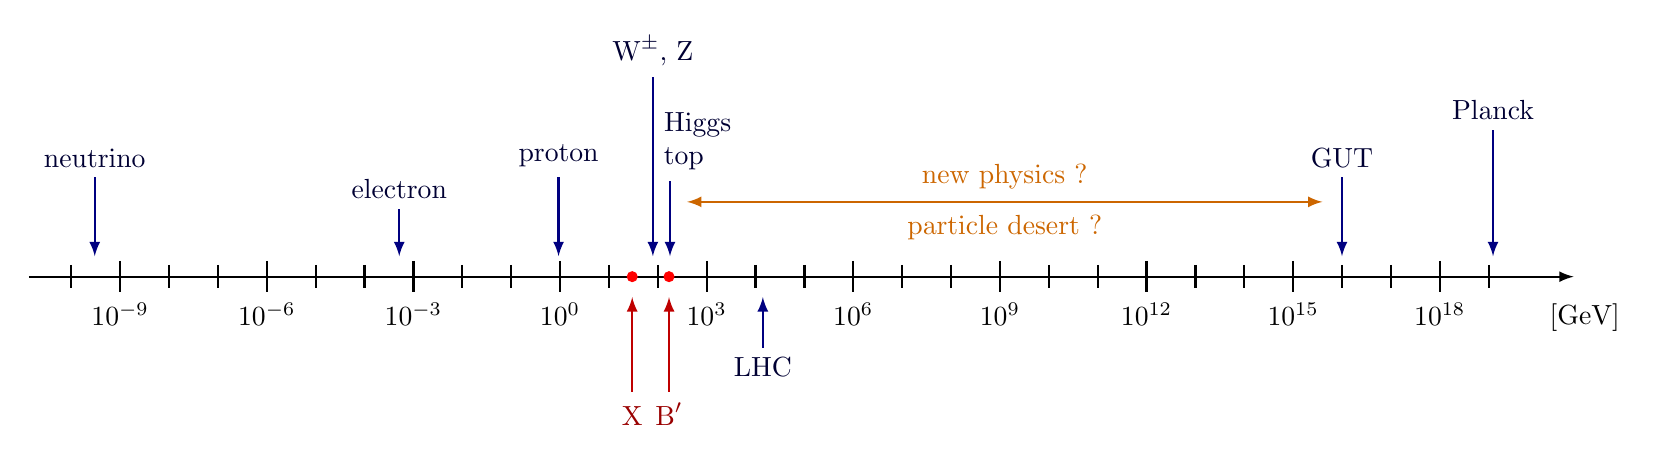
\begin{tikzpicture}[]
  
  % limits
  \newcount\nOne; \nOne=-10
  \def\w{18}      % width of axes
  \def\n{29}      % number of decades
  \def\noffset{1} % offset labels
  \def\nskip{3}   % skip number
  \def\la{2.00}   % arrow length
  \def\lt{0.20}   % tick length
  \def\ls{0.15}   % tick length (skipped)
  
  % help functions
  \def\myx(#1){{(#1-\nOne)*\w/\n}}
  \def\arrowLabel(#1,#2,#3,#4){
    \def\xy{(#1-\nOne)*\w/\n}; \pgfmathparse{int(#2*100)};
    \ifnum \pgfmathresult<0
      \def\yyp{{(\lt*(-0.10+#2))}}; \def\yyw{{(\yyp-\la*\lt*#3)}}
      \draw[<-,thick,black!50!blue,align=center]
        (\myx(#1),\yyp) -- (\myx(#1),\yyw)
        node[below,black!80!blue] {#4}; %,fill=white
    \else
      \def\yyp{{(\lt*(0.10+#2)}}; \def\yyw{{(\yyp+\la*\lt*#3)}}
      \draw[<-,thick,black!50!blue,align=center]
        (\myx(#1),\yyp) -- (\myx(#1),\yyw)
        node[above,black!80!blue] {#4};
    \fi}
  \def\arrowLabelRed(#1,#2,#3,#4){
    \def\yyp{{(\lt*(-0.10+#2))}}; \def\yyw{{(\yyp-\la*\lt*#3)}}
    \fill[red,radius=2pt] (\myx(#1),0) circle;
    \draw[<-,thick,black!25!red,align=center]
      (\myx(#1),\yyp) -- (\myx(#1),\yyw)
      node[below,black!40!red] {\strut#4}; %,fill=white
    }
  
  % axis
  \draw[->,thick] (-\w*0.03,0) -- (\w*1.06,0)
                  node[right=4pt,below=6pt] {[GeV]};
  
  % ticks
  \foreach \tick in {0,1,...,\n}{
    \def\x{{\tick*\w/\n}}
    \def\dec{\the\numexpr \nOne+\tick \relax}
	\pgfmathparse{Mod(\tick-\noffset,\nskip)==0?1:0}
	\ifnum\pgfmathresult>0
	  \draw[thick] (\x,\lt) -- (\x,-\lt) % ten tick
	               node[below] {$10^{\dec}$}; % label
	\else
      \draw[thick] (\x,\ls) -- (\x,-\ls); % ten tick
	\fi
  }
  
  % label
  \arrowLabel(-9.52,1.2,2.5,neutrino) % log(0.0000000003)=-9.523 (0.3 eV)
  \arrowLabel(-3.29,1.2,1.5,electron) % log(0.000510)=-3.292 (0.510 MeV)
  \arrowLabel(-0.03,1.2,2.5,proton)   % log(0.938)=-0.03
  \arrowLabel( 1.90,1.2,5.7,$\text{W}^\pm$, $\text{Z}$) % log(80)=1.90, log(90)=1.95
  \arrowLabel( 2.25,1.2,2.4,\qquad Higgs\\\quad top) % log(125)=2.10, log(175)=2.24
  \arrowLabel( 4.15,-1.2,1.6,LHC)     % log(1400)=4.146
  \arrowLabel(16.00,1.2,2.5,GUT)      % 10^25 eV = 10^16 GeV
  \arrowLabel(19.09,1.2,4.0,Planck)   % Planck % quantum gravity % 1.22x10^19 . GeV
  
  % low mass
  \arrowLabelRed(1.477,-1.2,3.0,X)    % ln(30) = 1.477
  \arrowLabelRed(2.230,-1.2,3.0,$\text{B}'$) % ln(170) = 2.230
  
  % stretch
  \draw[<->,thick,black!20!orange]
    ({(2.6-\nOne)*\w/\n},0.95) -- ({(15.6-\nOne)*\w/\n},0.95)
    node[midway,below=1pt] {particle desert ?}
    node[midway,above=1pt] {new physics ?};
  
\end{tikzpicture}






% TIMELINE - particle physics
% sources: http://web.ihep.su/dbserv/compas/src/
%          http://www.particleadventure.org/other/history/
%          https://en.wikipedia.org/wiki/Timeline_of_particle_discoveries
\large
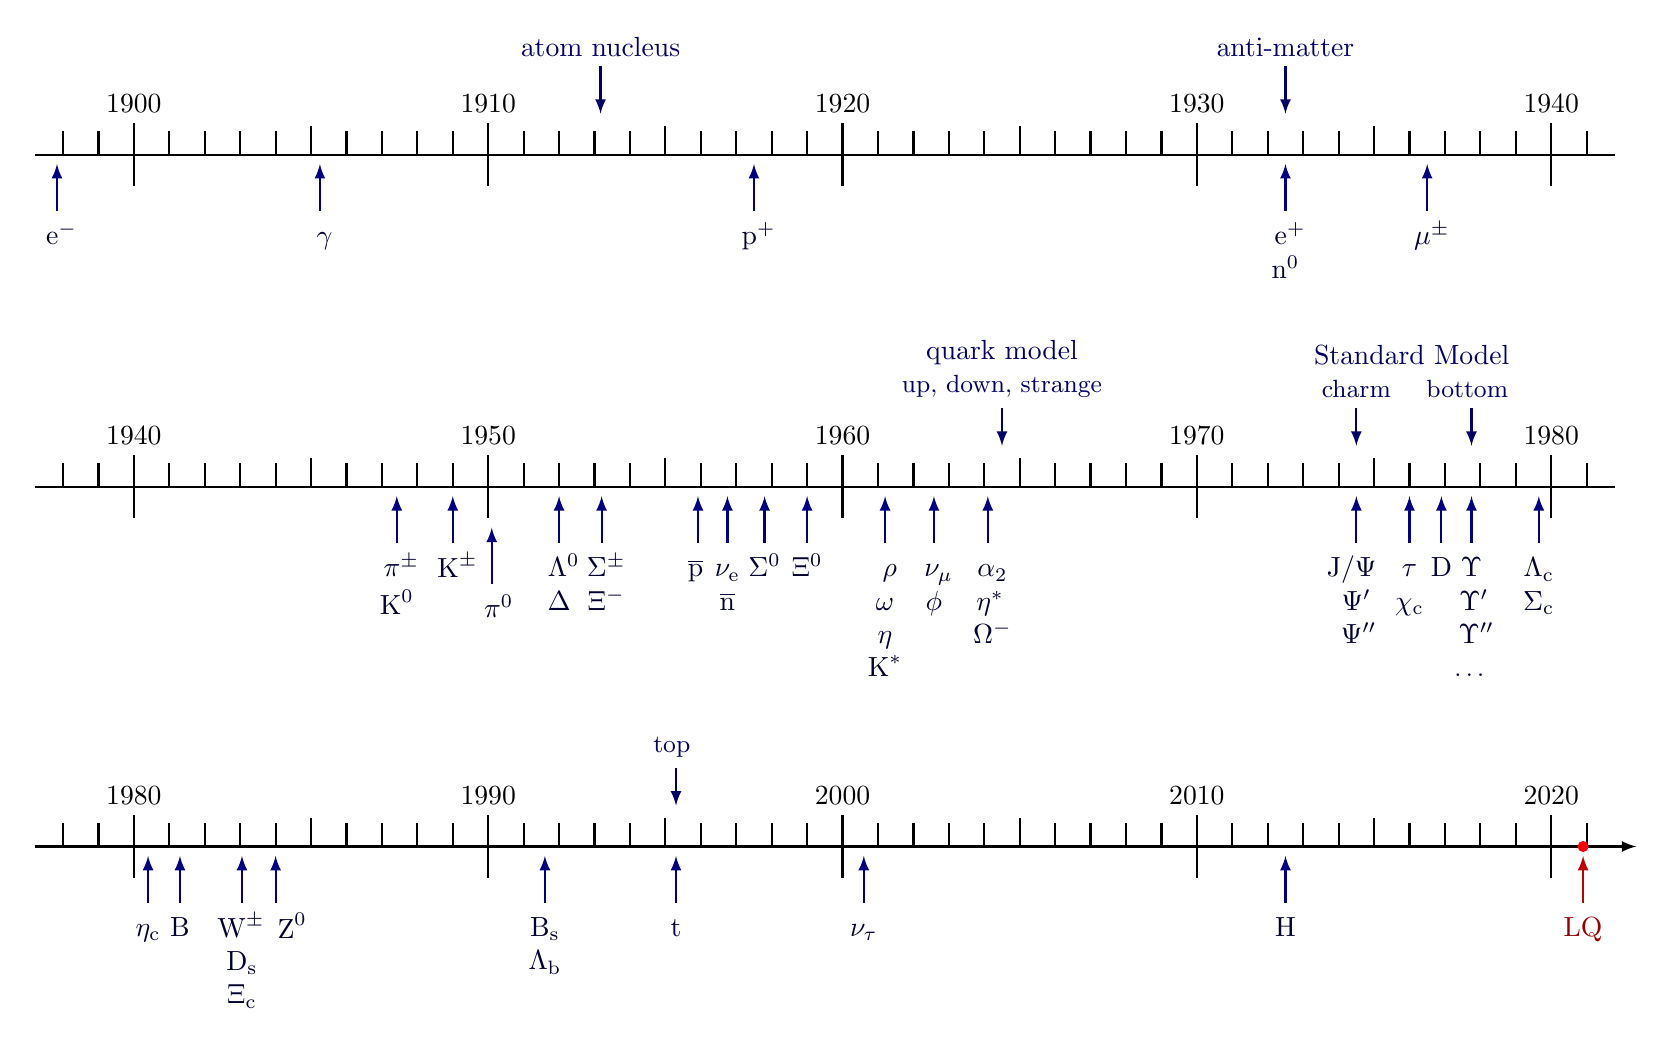
\begin{tikzpicture}[] %[minimum height=10pt, text height=10pt,text depth=10pt,

  % limits
  \newcount\yearOne; \yearOne=1900
  \newcount\yoffset;
  \def\w{18}       % width of axes
  \def\n{4}        % number of decades
  \def\lt{0.40}    %  ten tick length
  \def\lf{0.36}    % five tick length
  \def\lo{0.30}    %  one tick length
  \def\lext{0.07}  % left extension of axes
  \def\rext{1.045} % left extension of axes
  
  % help functions
  \def\yearLabel(#1,#2,#3){\node[above,black!60!blue] at ({(#1-\yearOne)*\w/\n/10},{\lt*#2}) {#3};}
  \def\yearArrowLabel(#1,#2,#3,#4){
    \def\xy{{(#1-\yearOne)*\w/\n/10}}; \pgfmathparse{int(#2*100)};
    \ifnum \pgfmathresult<0 % below
      \def\yyp{{(\lt*(0.90+#2))}}; \def\yyw{{(\yyp-\lt*#3)}}
      \draw[<-,thick,black!50!blue,align=center]
        (\xy,\yyp) -- (\xy,\yyw)
        node[below,black!80!blue] at (\xy,\yyw) {\strut #4};
    \else % under
      \def\yyp{{(\lt*(0.10+#2)}}; \def\yyw{{(\yyp+\lt*#3)}}
      \draw[<-,thick,black!60!blue,align=center]
        (\xy,\yyp) -- (\xy,\yyw)
        node[above] at (\xy,\yyw) {#4};
    \fi}
  \def\yearArrowLabelRed(#1,#2,#3,#4){
    \def\xy{{(#1-\yearOne)*\w/\n/10}}; \pgfmathparse{int(#2*100)};
      \def\yyp{{(\lt*(0.90+#2))}}; \def\yyw{{(\yyp-\lt*#3)}}
      \fill[red,radius=2pt] (\xy,0) circle;
      \draw[<-,thick,black!25!red,align=center]
        (\xy,\yyp) -- (\xy,\yyw)
        node[below,black!40!red] at (\xy,\yyw) {\strut #4};
     }  
  
  
  %---------------%
  %  1900 - 1940  %
  %---------------%
  
  % axis
  \draw[thick] (-\w*0.07,0) -- (\w*\rext,0);
  
  % ticks
  \foreach \tick in {0,1,...,\n}{
    \def\x{{\tick*\w/\n}}
    \def\year{\the\numexpr \yearOne+\tick*10 \relax}
    \draw[thick] (\x,-\lt) -- (\x,\lt) % ten tick
                 node[above] {\year};
	
	\ifnum \tick<\n
      \draw[thick] ({(\x+\w/\n/2)},0) -- ({(\x+\w/\n/2)},\lf); % five tick
      \foreach \ticko in {1,2,3,4,6,7,8,9}{
        \def\xo{{(\x+\ticko*\w/\n/10)}}
  	    \draw[thick] (\xo,0) -- (\xo,\lo);  % one tick
	}\fi
  }
  
  % extra ticks
  \draw[thick] (-1*\w/\n/10,0) -- (-1*\w/\n/10,\lo);
  \draw[thick] (-2*\w/\n/10,0) -- (-2*\w/\n/10,\lo);
  \draw[thick] ({\w+\w/\n/10},0) -- ({\w+\w/\n/10},\lo);
  
  % labels
  \yearArrowLabel(1897.83,-1.2,1.5,
                  $\text{e}^-$)      % electron 10/1897 Thomson
  \yearArrowLabel(1905.25,-1.2,1.5,
                  $\gamma$)          % photon   03/1905 Einstein
  \yearArrowLabel(1913.17, 1.2,1.5,
                  atom nucleus)      % nucleus  02/1913 Rutherford
  \yearArrowLabel(1917.50,-1.2,1.5,
                  $\text{p}^+$)      % proton      1917 Rutherford (Philos. Mag., Ser. 6, Vol. 37, 581 (1919))
  \yearArrowLabel(1932.50, 1.2,1.5,
                  anti-matter)       % anti-matter
  \yearArrowLabel(1932.50,-1.2,1.5,
                  $\text{e}^+$\\     % positron    1932 Anderson
                  $\text{n}^0$)      % neutron     1932 Chadwick
  \yearArrowLabel(1936.50,-1.2,1.5,
                  $\mu^\pm$)         % muon        1936
  
  
  %---------------%
  %  1940 - 1980  %
  %---------------%
  
  \yearOne=1940; \advance\yoffset by 120
  \begin{scope}[yshift=-\yoffset]
    
    % axis
    \draw[thick] (-\w*\lext,0) -- (\w*\rext,0);
    
    % ticks
    \foreach \tick in {0,1,...,\n}{
      \def\x{{\tick*\w/\n}}
      \def\year{\the\numexpr \yearOne+\tick*10 \relax}
      \draw[thick] (\x,-\lt) -- (\x,\lt) % ten tick
	               node[above] {\year};
      \ifnum \tick<\n
        \draw[thick] ({(\x+\w/\n/2)},0) -- ({(\x+\w/\n/2)},\lf); % five tick
        \foreach \ticko in {1,2,3,4,6,7,8,9}{
          \def\xo{{(\x+\ticko*\w/\n/10)}}
  	      \draw[thick] (\xo,0) -- (\xo,\lo);  % one tick
	  }\fi
    }

    % extra ticks
    \draw[thick] (-1*\w/\n/10,0) -- (-1*\w/\n/10,\lo);
    \draw[thick] (-2*\w/\n/10,0) -- (-2*\w/\n/10,\lo);
    \draw[thick] ({\w+\w/\n/10},0) -- ({\w+\w/\n/10},\lo);
  
    % labels
    \yearArrowLabel(1947.42,-1.2,1.5,
                    $\pi^\pm$\\            % pions    05/1947 Lattes, Muirhead, Occhialini, Powell
                    $\text{K}^0$)          % neutral kaons 12/1947 Rochester & Butler, Nature, 160, 855
    \yearArrowLabel(1949.00,-1.2,1.5,
                    $\text{K}^\pm$)        % kaons    12/1949 Powell, Fowler, Perkins, Nature, 163, 82
    \yearArrowLabel(1950.10,-2.2,1.8,
                  \,$\pi^0$)               % pi0      01/1950 Caltech
    \yearArrowLabel(1952.00,-1.2,1.5,
                    $\Lambda^0$\\          % Lambda0  12/1950 Hopper, Biswas, Phys. Rev. 80, 1099
                    $\Delta$)              % 1952 Anderson, Fermi, (Chicago Cyclotron), Phys. Rev., 85, 936
                                           % 1956 Ashkin (Rochester cyclotron), Phys. Rev., 101, 1149
     % Sigma+ 1953 Bonetti, Nuovo Cimento, 10, 1; Danysz, Pniewski, Phil. Mag., 44, 348; Cosmotron Brookhaven, Phys. Rev., 93, 109
     % Xi- "negative hyperon" 1954 Cowan (Caltech), Phys. Rev., 94, 161
    \yearArrowLabel(1953.20,-1.2,1.5,\,\,$\Sigma^\pm$\\\,\,$\Xi^-$)
    \yearArrowLabel(1955.92,-1.2,1.5,$\overline{\text{p}}$\,) % 11/1955 Chamberlain, Segrè (Bevatron) Phys. Rev. 100, 947
    \yearArrowLabel(1956.75,-1.2,1.5,$\nu_\text{e}$\\$\overline{\text{n}}$) % 09/1956 Reines, Cowan, Nature, 178, 446
    \yearArrowLabel(1957.80,-1.2,1.5,$\Sigma^0$) % 
    \yearArrowLabel(1959.00,-1.2,1.5,$\Xi^0$) % Xi 1959 (1964 Brookhaven)
    % 1960  Sigma*(1385) Phys. Rev. Lett., 5, 520
    \yearArrowLabel(1961.20,-1.2,1.5,
                    $\rho$\\            % 1961 Erwin (Cosmotron) Phys. Rev. Lett., 6, 628
                    $\omega$\\          % 1961 Maglic, Alvarez, Phys. Rev. Lett., 7, 178
                    $\eta$\\            % 1961 Pevsner, Phys. Rev. Lett., 7, 421
                    $\text{K}^*$)       % 1961 Alston, Phys. Rev. Lett., 6, 300, 1962 Phys. Rev. Lett., 9, 330
    % 19.. strangeness "associated-production", Pais
    % 1962 Eightfold Way, Gell-Man
    \yearArrowLabel(1962.58,-1.2,1.5,\vspace{2pt}
                    $\nu_\mu$\\         % 07/1962, Ledderman, Danby, Phys. Rev. Lett. 9, 36
                    $\phi$)             % 1962, Pjerrou Phys. Rev. Lett., 9, 114, Bertanza, Phys. Rev. Lett., 9, 180
    % 1962 f particle?
    \yearArrowLabel(1964.10,-1.2,1.5,
                    $\alpha_2$\\        %
                    \,$\eta^*$\\        %
                    \,\,$\Omega^-$)     % 02/1964, Barnes, Brookhaven, Phys. Rev. Lett. 12, 204
    \yearArrowLabel(1964.50, 1.2,1.2,
                    quark model\\
                    \small{up, down, strange}) % Gell-Mann
    % 1967 Steven Weinberg, Abdus Salam: electroweak unification
    \yearArrowLabel(1974.50, 1.2,1.2,
                    \qquad\qquad Standard Model\\
                    \small{charm})     % charm
    % 1974 November Revolution
    \yearArrowLabel(1974.50,-1.2,1.5,$\text{J/}\Psi$\,\,\\$\Psi'$\\\,$\Psi''$) % 
    %\yearLabel(1973,4.0,Standard Model) % Standard Model
    % tau 1975 Perl, Abrams, Phys. Rev. Lett. 35, 1489
    \yearArrowLabel(1976.00,-1.2,1.5,$\tau$\\$\chi_\text{c}$) % 
    \yearArrowLabel(1976.90,-1.2,1.5,
                    $\text{D}$        ) % 1976 SLAC
    \yearArrowLabel(1977.75, 1.2,1.2,
                    \small{bottom} )    % bottom
    \yearArrowLabel(1977.75,-1.2,1.5,$\Upsilon$\\\,$\Upsilon'$\\\,\,$\Upsilon''$\\\small\ldots) % Fermilab
    \yearArrowLabel(1979.65,-1.2,1.5,$\Lambda_\text{c}$\\$\Sigma_\text{c}$) % 
    
  \end{scope}
  
  
  %---------------%
  %  1980 - 2020  %
  %---------------%
  
  \yearOne=1980; \advance\yoffset by 130
  \begin{scope}[yshift=-\yoffset]
    
    % axis
    \draw[->,thick] (-\w*\lext,0) -- (\w*1.06,0);
    
    % ticks
    \foreach \tick in {0,1,...,\n}{
      \def\x{{\tick*\w/\n}}
      \def\year{\the\numexpr \yearOne+\tick*10 \relax}
      \draw[thick] (\x,-\lt) -- (\x,\lt) % ten tick
	               node[above] {\year};
      \ifnum \tick<\n
        \draw[thick] ({(\x+\w/\n/2)},0) -- ({(\x+\w/\n/2)},\lf); % five tick
        \foreach \ticko in {1,2,3,4,6,7,8,9}{
          \def\xo{{(\x+\ticko*\w/\n/10)}}
  	      \draw[thick] (\xo,0) -- (\xo,\lo);  % one tick
	  }\fi
    }
    
    % extra ticks
    \draw[thick] (-1*\w/\n/10,0) -- (-1*\w/\n/10,\lo);
    \draw[thick] (-2*\w/\n/10,0) -- (-2*\w/\n/10,\lo);
    \draw[thick] ({\w+\w/\n/10},0) -- ({\w+\w/\n/10},\lo);
  
    % labels
    \yearArrowLabel(1980.40,-1.2,1.5,
                    $\eta_\text{c}$   )  % 
    \yearArrowLabel(1981.30,-1.2,1.5,
                    B                 )  % 
    \yearArrowLabel(1983.05,-1.2,1.5,
              \mbox{$\text{W}^\pm$\hspace{4pt}}\\
                    $\text{D}_\text{s}$\\
                    $\Xi_\text{c}$    )  % 
    \yearArrowLabel(1984.00,-1.2,1.5,
              \mbox{\hspace{12pt}$\text{Z}^0$} ) % 
    \yearArrowLabel(1991.60,-1.2,1.5,$\text{B}_\text{s}$\\$\Lambda_\text{b}$)  % Bs Fermilab
    \yearArrowLabel(1995.30,-1.2,1.5,t)  % 
    \yearArrowLabel(1995.30, 1.2,1.2,
                    \small{top}      )   %  
    \yearArrowLabel(2000.60,-1.2,1.5,$\nu_\tau$)  % 
    \yearArrowLabel(2012.50,-1.2,1.5,H)  % 
    %\yearArrowLabelRed(2017.7,-1.2,1.5,X\\\,$\text{B}'$) % low mass
    \yearArrowLabelRed(2020.9,-1.2,1.5,LQ) % leptoquark
    
  \end{scope}
  
  
\end{tikzpicture}



\end{document}